\documentclass{beamer}
\mode<presentation>
{
\usetheme{Boadilla}
%\setbeamercovered{transparent}
%\useoutertheme{smoothbars}
}
%\addtobeamertemplate{footline}{\insertframenumber/\inserttotalframenumber}

\usepackage[utf8]{inputenc} \usepackage[english]{babel}
\usepackage{graphicx} \usepackage{geometry}
\usepackage{pifont}
\usepackage{hyperref}
\usepackage{tikz}
\usepackage{fancyvrb}
\DefineVerbatimEnvironment{verbatim}{Verbatim}{formatcom=\color{blue}}
%\usepackage{minted}

%\newminted{python}{fontsize=\scriptsize,linenos}
%\newminted{python3}{fontsize=\tiny,linenos}

 
\newcommand{\E}[1]{{\textbf{#1}}}
\newcommand{\C}[1]{{\color{red}\texttt{#1}}}
\definecolor{mygreen}{cmyk}{0.888,0,0.888,0.298}
\definecolor{mblue}{RGB}{0,34,102}
\definecolor{mred}{RGB}{205,0,0}
\definecolor{mcc}{RGB}{65,105,225}
\newcommand{\G}[1]{{\color{mygreen}{#1}}}
\newcommand{\B}[1]{{\color{blue}{#1}}}
\newcommand{\ar}{\ding{220} }
\newcommand{\todo}[1]{{\colorbox{yellow}{\color{fg}#1}}}


\title{VM5k and DVMS on Grid'5000}
\subtitle{Deploying and Managing Thousands of Virtual Machines on Hundreds of Nodes Distributed Geographically}

% - Use the \inst{?} command only if the authors have different
%   affiliation.
%\author{F.~Author\inst{1} \and S.~Another\inst{2}}
\author[J. Pastor and L. Pouilloux]{Jonathan Pastor\inst{1} \and Laurent Pouilloux\inst{2}}

% - Use the \inst command only if there are several affiliations.
% - Keep it simple, no one is interested in your street address.
\institute[Hemera]
{
\inst{1}%
Hemera Phd\\
ASCOLA - Mines Nantes / Inria
\and
\inst{2}%
Hemera Engineer\\
Inria / ENS Lyon}
 
\date[G5K School 2014]{18-06-2014 / Grid'5000 School}


% This is only inserted into the PDF information catalog. Can be left
% out.
\subject{VM5K_DVMS}



% If you have a file called "university-logo-filename.xxx", where xxx
% is a graphic format that can be processed by latex or pdflatex,
% resp., then you can add a logo as follows:

%\pgfdeclareimage[height=0.5cm]{university-logo}{logo_inria.jpg}
%\logo{\pgfuseimage{university-logo}}


\begin{document}

\begin{frame}
\titlepage
\end{frame}


\begin{frame}{Context}
Cloud computing usage is becoming very popular.
\begin{itemize}
    \item Ever-increasing demand $\Rightarrow$ ever-increasing
infrastructure size.
    \item Problems: scalability, reliability, network overhead, energy 
    but also security and juridiction
\end{itemize}
\begin{block}{Proposition: [Greenberg2009]} 
Concept of microdatacenters geographically spread 
\end{block}
\end{frame}


\begin{frame}{Discovery project}
\framesubtitle{http://beyondtheclouds.github.io/}
Decentralise the production of computing ressources
\begin{itemize}
    \item Chord topology 
    \item taking into account network distance
\end{itemize}
\begin{minipage}{0.63\linewidth}
\includegraphics[width=0.9\linewidth]{dvms1.png}
\end{minipage}
\hfill
\begin{minipage}{0.33\linewidth}
\includegraphics[width=0.9\linewidth]{dvms_vivaldi.png}
\end{minipage}
\begin{block}{}
Evaluating DVMS with Vivaldi (coordinates system)
\end{block} 
\end{frame}


{
\usebackgroundtemplate{%
\tikz[overlay,remember picture] \node[opacity=1, at=(current page.center)] {
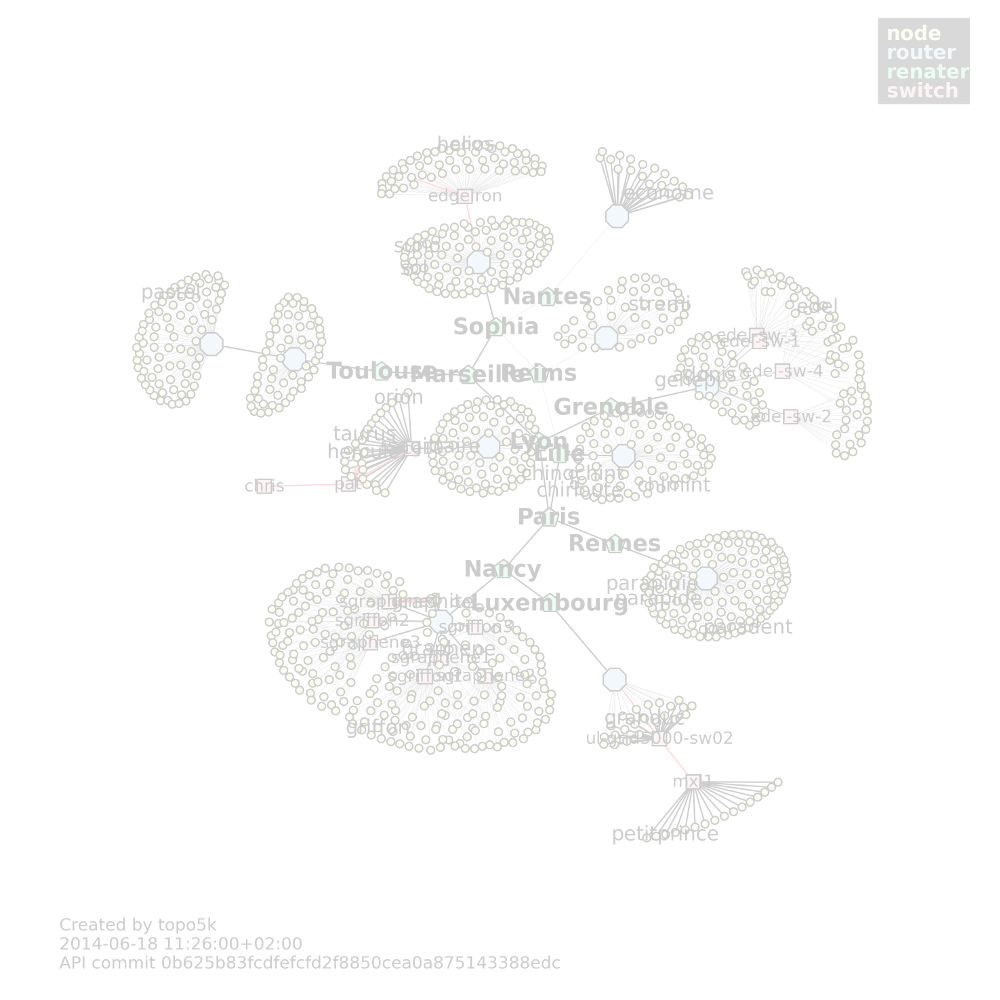
\includegraphics[height=0.9\paperheight,width=0.9\paperwidth,keepaspectratio]{topo5k.png}};
}
\begin{frame}{Grid'5000 as a testbed}
\begin{itemize}
    \item 10Gb interconnected network
    \item various hardware (cpu, memory size, disks, network bandwidth)
    \item KaVLAN: allow to have a single network over the sites
    \item full experiment stack control (hardware, OS, hypervisor)
\end{itemize}
\end{frame}
}


\begin{frame}{Experimental Workflow}
\begin{enumerate}
    \item reserve many nodes on different sites, with a global-KaVLAN
    \item deploy thousants of Virtual Machines
    \item initiate stress process on them
    \item install DVMS
    \item use vivaldi to compute hosts distances
    \item generate random stress on the virtual machines
    \item live experiment visualization
    \item collect results
\end{enumerate}
\end{frame}

\begin{frame}[fragile]{(F)ind yo(U)r (N)ode on g5(K)}
\framesubtitle{A advanced resources discovery tool for multisite reservation}
\small
\begin{verbatim}
funk -m free -r grid5000:200 -o "-t deploy" -w 12:00:00 
  -b helios,sagittaire,nantes,reims,graphite -k -c
\end{verbatim}
\begin{center}
\includegraphics[height=0.7\paperheight,width=0.7\paperwidth,keepaspectratio]{funk_slots.png}
\end{center}
\end{frame}

 
\begin{frame}{Automatic Virtual Machines deployment}
\framesubtitle{Moving FLauncher (D. Balouek and F. Quesnel) to vm5k}
\begin{center}
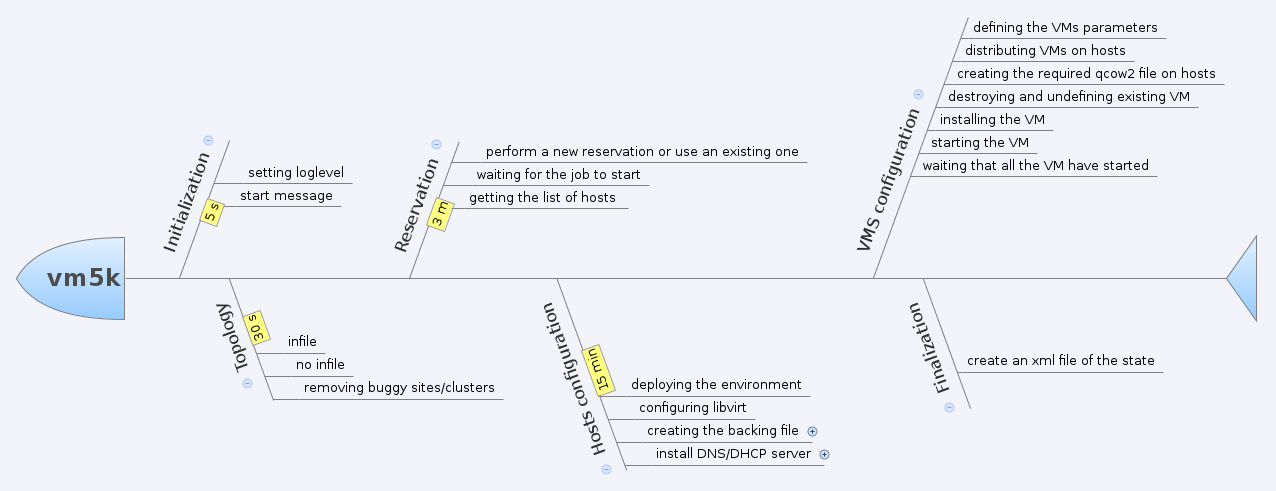
\includegraphics[height=0.6\paperheight,keepaspectratio]{vm5k_workflow.png}
\end{center}
\begin{alertblock}{}
Tested successfully up to 5 000 VMs on 300 nodes.
\end{alertblock}
\end{frame}

\begin{frame}[fragile]{Stress initialization}
On all running Virtual Machines and using \href{http://execo.gforge.inria.fr/doc/latest-stable/userguide.html}{execo}
\begin{itemize}
    \item upload the \verb=memtouch= binary
    \item start a memtouch process
    \item set it's cpu usage to 1\% using \verb=cpulimit=
\end{itemize}
\begin{alertblock}{}
All VMs are ready to be stressed.
\end{alertblock}

\end{frame}

\begin{frame}{Vivaldi}

\end{frame}

\begin{frame}{DVMS}

\end{frame}

\begin{frame}{Live visualization}
\begin{center}
    \url{http://localhost:9000}
\end{center}
\begin{itemize}
    \item migration count
    \item infrastructure state (VM position and load) 
    \item distance map from Vivaldi (used by DVMS to determine where to migrate the VMs)
    \item bonus: node live power usage
\end{itemize}
\end{frame}
    
\begin{frame}[fragile]{Load events generation}
We can tune:
\begin{itemize}
    \item distribution of event load value
    \item events frequency
\end{itemize}
\tiny
\begin{verbatim}
<?xml version="1.0" encoding="UTF-8"?>
<events>
  <event type="update_cpu_load" time="0.6322858606354911" target="vm-103" location="10.27.216.103" value="30"/>
  <event type="update_cpu_load" time="0.6501133097844356" target="vm-24" location="10.27.216.24" value="50"/>
  <event type="update_cpu_load" time="0.77156495657007" target="vm-59" location="10.27.216.59" value="100"/>
  <event type="update_cpu_load" time="1.001639188886804" target="vm-123" location="10.27.216.123" value="80"/>
  <event type="update_cpu_load" time="1.7390251934205876" target="vm-19" location="10.27.216.19" value="100"/>
  <event type="update_cpu_load" time="2.161792297887189" target="vm-44" location="10.27.216.44" value="80"/>
  <event type="update_cpu_load" time="3.1211590695284515" target="vm-41" location="10.27.216.41" value="100"/>
  <event type="update_cpu_load" time="3.525741904535117" target="vm-61" location="10.27.216.61" value="40"/>
 ...
</events>
\end{verbatim}
\begin{block}{}
\normalsize
Use an execo script to set the value of the load using \verb=cpulimit=
\end{block}
\end{frame}


\begin{frame}{Results Analysis}
\begin{itemize}
    \item Vivaldi map
    \item Migration statistics
    \item Bonus: fine-grained power consumption for some nodes
\end{itemize}
\end{frame}

\begin{frame}{Conclusion}
Large scale validation of DVMS taking into account node distance
\begin{itemize}
    \item -almost- fully automatized experiment
    \item wide usage of Grid'5000 features (API, Kadeploy, KaVLAN, Kwapi)
    \item real execution up to 5000 Virtual Machines
    \item demo available on \href{https://www.grid5000.fr/mediawiki/index.php/Challenge_DVMS_Live_-_School_2014}
    {Challenge\_DVMS\_Live\_-\_School\_2014}
\end{itemize}

\begin{block}{}
\small
Jonathan Pastor, Marin Bertier, Frédéric Desprez, Adrien Lèbre, Flavien Quesnel, 
and Cédric Tedeschi. \textit{Locality-aware Cooperation for VM Scheduling in 
Distributed Clouds}. In Euro-Par 2014, Porto, Portugal, August 2014.
\end{block}
\end{frame}

\begin{frame}
Thank your for your attention. Questions ?
\end{frame}

\end{document}
